\documentclass{jib}
\newlength{\platz}
\setlength{\platz}{15pt}
\RequirePackage{listings}

%\usepackage{changepage} %test, TODO remove

\lstset{%
  basicstyle=\ttfamily,
  fontadjust,
  flexiblecolumns=true,
  frame=L,
  xleftmargin=15pt,
  framesep=5pt,
  emphstyle=\rmfamily\itshape}
  

%%%%%%%%%%%%%%%%%%%%%%%%%%%%%%%%%%%%%%%%%%%%%%%%%%%%%%%%%%
% JIB Header/Footer
%%%%%%%%%%%%%%%%%%%%%%%%%%%%%%%%%%%%%%%%%%%%%%%%%%%%%%%%%%
\jibvolume{XX} % insert volume
\jibissue{X}   % insert issue
\jibpages{XXX} % insert article ID
\jibyear{XXXX} % insert year
\makeHeaderFooter{} % leave as is
%%%%%%%%%%%%%%%%%%%%%%%%%%%%%%%%%%%%%%%%%%%%%%%%%%%%%%%%%%

\usepackage{pdfpages}

\begin{document}

%%%%%%%%%%%%%%%%%%%%%%%%%%%%%%%%%%%%%%%%%%%%%%%%%%%%%%%%%%
%
% Title Page
%
%%%%%%%%%%%%%%%%%%%%%%%%%%%%%%%%%%%%%%%%%%%%%%%%%%%%%%%%%%

\begin{jibtitlepage}

\jibtitle{Synthetic Biology Open Language (SBOL) Version 3.1.0}


%We did not provide author(s) nor author footnote(s), please complete as applicable.
% Please make sure to use unique footnote characters for each author
\jibauthor{Lukas Buecherl\iref{cu},
           Thomas Mitchell\iref{bbn},
           James Scott-Brown\iref{ue},
           Prashant Vaidyanathan\iref{ob},
           Gonzalo Vidal\iref{nu},
%         
           Hasan Baig\iref{uc},
           Bryan Bartley\iref{bbn},
           Jacob Beal\iref{bbn},
           Matthew Crowther\iref{nu},
           Pedro Fontanarrosa\iref{cu},
           Thomas Gorochowski\iref{ub},
           Raik Gr\"unberg\iref{kaust},
           Vishwesh Kulkarni\iref{uw},
           James McLaughlin\iref{nu},
           G\"{o}ksel M{\i}s{\i}rl{\i}\iref{keele},
           Ernst Oberortner\iref{jgi},
           Anil Wipat\iref{nu},
%
           and
           Chris Myers\iref{cu}
           }

\addjibinstitution{cu}{University of Colorado Boulder, USA}
\addjibinstitution{bbn}{Raytheon BBN Technologies, USA}
\addjibinstitution{ue}{University of Edinburgh, UK}
\addjibinstitution{ob}{Oxford Biomedica, UK}
\addjibinstitution{nu}{Newcastle University, UK}
\addjibinstitution{uc}{University of Connecticut, USA}
\addjibinstitution{ub}{University of Bristol, UK}
\addjibinstitution{kaust}{King Abdullah University for Science and Technology, SA}
\addjibinstitution{uw}{University of Warwick, UK}
\addjibinstitution{keele}{Keele University, UK}
\addjibinstitution{jgi}{DOE Joint Genome Institute, USA}



\end{jibtitlepage}

% The abstract
\begin{abstract}
Synthetic biology builds upon genetics, molecular biology, and metabolic engineering by applying engineering principles to the design of biological systems. When designing a synthetic system, synthetic biologists need to exchange information about multiple types of molecules, the intended behavior of the system, and actual experimental measurements. The \emph{Synthetic Biology Open Language} (SBOL) has been developed as a standard to support the specification and exchange of biological design information in synthetic biology, following an open community process involving both bench scientists and scientific modelers and software developers, across academia, industry, and other institutions. 
This document describes SBOL 3.1.0, which improves on version 3.0.0 by including a number of corrections and clarifications as well as several other updates and enhancements.  First, this version includes a complete set of validation rules for checking whether documents are valid SBOL 3.  Second, the best practices section has been moved to an online repository that allows for more rapid and interactive of sharing these conventions.  Third, it includes updates based upon six community approved enhancement proposals. Two enhancement proposals are related to the representation of an object's namespace.  In particular, the \textbf{Namespace} class has been removed and replaced with a \textbf{namespace} property on each class.  Another enhancement is the generalization of the \textbf{CombinatorialDeriviation} class to allow direct use of \textbf{Features} and \textbf{Measures}.  Next, the \textbf{Participation} class now allow \textbf{Interactions} to be \textbf{participants} to describe higher-order interactions.  Another change is the use of \emph{Sequence Ontology} terms for \textbf{Feature} \textbf{orientation}.  Finally, this version of SBOL has generalized from using \emph{Unique Reference Identifiers} (URIs) to \emph{Internationalized Resource Identifiers} (IRIs) to support international character sets.

%Rewrite:\\
%For the updated specification SBOL 3.1, six enhancement protocols (SEPs) were accepted: SEP 047 changes the direction of the Namespace references. Instead of Namespaces pointing to objects, objects should point to their Namespace. The Namespace object will no longer be a subclass of Collection. Instead, it will be a subclass of TopLevel, with no members property. Building on top of SEP 047, SEP 050 removes the Namespace object, as its function has become largely obsolete. The TopLevel object will have a new hasNamespace property that is REQUIRED and is of type URI. SEP 048 proposes a generalization of the CombinatorialDerivation class to allow direct use of all features and measures. The range of the VariableComponent property variable is changed from SubComponent to Feature. A new variantMeasure property is added to VariableComponent, with cardinality 0..n (i.e., optional, and as many as desired can be added).
%Given a set of values linked from a VariableComponent, it SHOULD be the case that all values are of type Measure or else all values are of type Feature. At present, it is explicitly left undefined how an algorithm ought to handle mixtures of Measure and Feature values. With SEP 049 SBOL now allows Participation objects to include interactions as higher-order participants. An interaction can now be a participant in another interaction, thereby allowing the higher-order interaction to be represented directly and transparently. The SBOL specification follows the general principle of reusing existing identifiers where possible, and only introducing own identifiers when necessary. SEP 053 introduces existing SO terms for Feature orientation. Finally, with SEP 056 the specification generalizes from URIs to IRIs.



%1. Abstract goes here.\\
%2. Also updated SBOL3.pdf after PRs have been accepted \\
%3. 61 one differences but not all worth mentioning \\
%4. Check releases \\

%Synthetic biology builds upon the techniques and successes of genetics, molecular biology, and metabolic engineering by applying engineering principles to the design of biological systems. The field still faces substantial challenges, including long development times, high rates of failure, and poor reproducibility. 
%One method to ameliorate these problems would be to improve the exchange of information about designed systems between laboratories. The \emph{Synthetic Biology Open Language} (SBOL) has been developed as a standard to support the specification and exchange of biological design information in synthetic biology, filling a need not satisfied by other pre-existing standards. This document details version 2.2.0 of SBOL that builds upon version 2.1.0 published in last year's JIB special issue.  In particular, SBOL 2.2.0 includes improved description and validation rules for genetic design provenance, an extension to support combinatorial genetic designs, a new class to add non-SBOL data as attachments, a new class for genetic design implementations, and a description of a methodology to describe the entire design-build-test-learn cycle within the SBOL data model.

%, introducing a standardized format for the electronic exchange of information on the structural and functional aspects of biological designs. The standard has been designed to support the explicit and unambiguous description of biological designs by means of a well defined data model. The standard also includes rules and best practices on how to use this data model and populate it with relevant design details. The publication of this specification is intended to make these capabilities more widely accessible to potential developers and users in the synthetic biology community and beyond.

\end{abstract}

This document does not contain technology or technical data controlled under either the U.S. International Traffic in Arms Regulations or the U.S. Export Administration Regulations.

% Include your PDF document
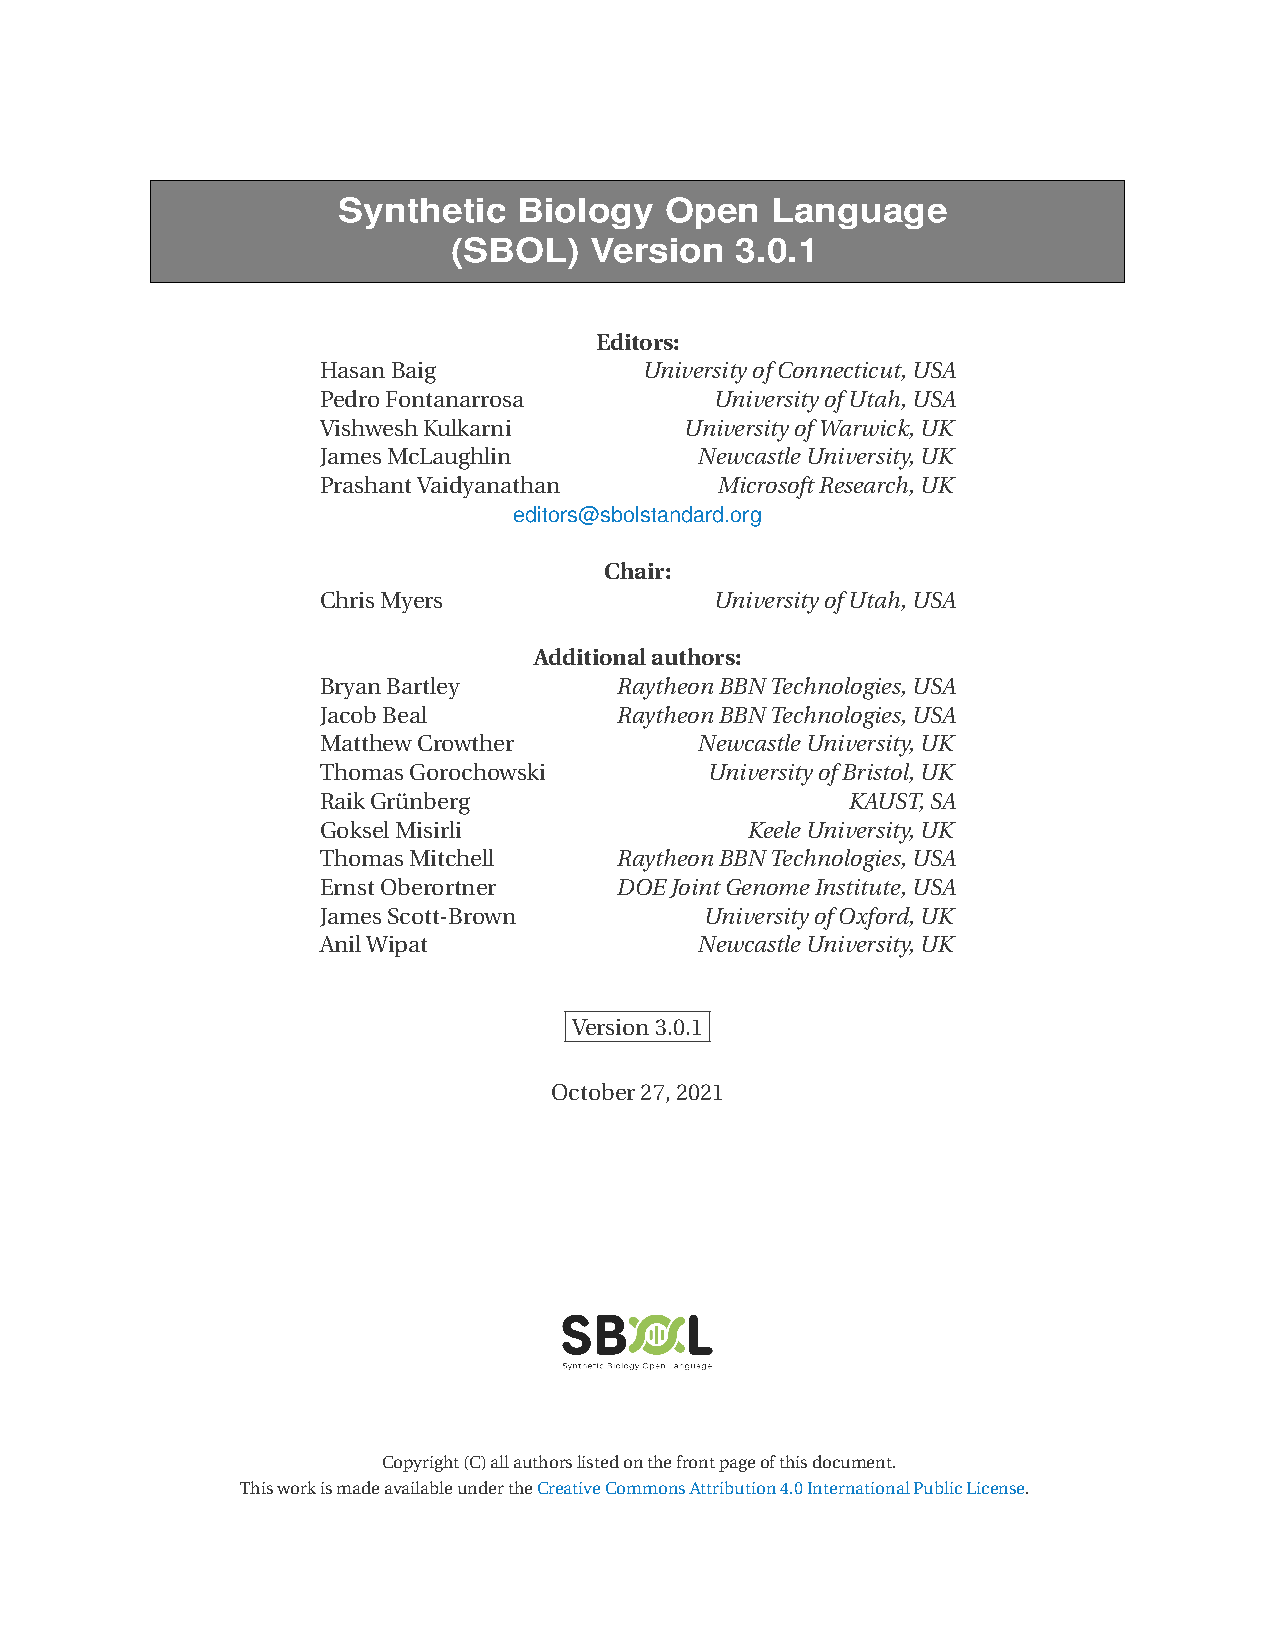
\includepdf[pages=-, offset=80 -80]{sbol3.pdf}

\end{document}